\documentclass[xcolor={table}]{beamer}
\usepackage{fleqn}
\usepackage{graphicx}
\usepackage{coordsys} %for \numbline commander

%Setup appearance:
\usetheme{Darmstadt}
\usefonttheme[onlylarge]{structurebold}
\setbeamerfont*{frametitle}{size=\normalsize,series=\bfseries}
\setbeamertemplate{navigation symbols}{}
\setbeamertemplate{bibliography item}{[\theenumiv]}

% Standard packages
\usepackage[english]{babel}
\usepackage[latin1]{inputenc}
\usepackage{times}
\usepackage[T1]{fontenc}
\usepackage{multirow}
\usepackage{subfigure}
\usepackage{pbox}
\usepackage{arydshln}
\usepackage{pifont}
\usepackage{cancel}
\usepackage{rotating} % for sideways headings

% Source Code packages
\usepackage{algorithm2e}
\usepackage{algorithmic}

\DeclareSymbolFont{extraup}{U}{zavm}{m}{n}
\DeclareMathSymbol{\varclub}{\mathalpha}{extraup}{84}
\DeclareMathSymbol{\varspade}{\mathalpha}{extraup}{85}
\DeclareMathSymbol{\varheart}{\mathalpha}{extraup}{86}
\DeclareMathSymbol{\vardiamond}{\mathalpha}{extraup}{87}

%%% This section command that adds a big page with section dividers
\usepackage{xifthen}% provides \isempty test
\newcommand{\SectionSlide}[2][]{
	\ifthenelse{\isempty{#1}}
		{\section{#2}\begin{frame} \begin{center}\begin{huge}#2\end{huge}\end{center}\end{frame}}
		{\section[#1]{#2}\begin{frame} \begin{center}\begin{huge}#2\end{huge}\end{center}\end{frame}}
}
%Extends the section slide to to include a shortened section title for the navigation bar as a second parameter
\newcommand{\SectionSlideShortHeader}[3][]{
	\ifthenelse{\isempty{#1}}
		{\section[#3]{#2}\begin{frame} \begin{center}\begin{huge}#2\end{huge}\end{center}\end{frame}}
		{\section[#1]{#2}\begin{frame} \begin{center}\begin{huge}#3\end{huge}\end{center}\end{frame}}
}

\newcommand{\refer}[1]{\footnote{#1}}
\newcommand{\GW}{\text{\textit{Guess-Who~}}}
\newcommand{\keyword}[1]{\alert{\textbf{#1}}\index{#1}}
\newcommand{\firstkeyword}[1]{\textbf{#1}\index{#1}}
\newcommand{\indexkeyword}[1]{\alert{\textbf{#1}\index{#1}}}
\newcommand{\featN}[1]{\textsc{#1}}
\newcommand{\featL}[1]{\textit{'#1'}}
 \newcommand{\ourRef}[1]{\ref{#1} $^{\text{\tiny[\pageref{#1}]}}$}
 \newcommand{\ourEqRef}[1]{\eqref{#1}$^{\text{\tiny[\pageref{#1}]}}$}
  
\DeclareMathOperator*{\argmax}{argmax}
\DeclareMathOperator*{\argmin}{argmin}

\title{Probability-based Learning\\Sections $6.4, 6.5$}
	\author{John D. Kelleher and Brian Mac Namee and Aoife D'Arcy}
	\institute{}
	\date{}

\begin{document}
\begin{frame}
	\titlepage
\end{frame}
\begin{frame}
	 \tableofcontents
\end{frame}


\SectionSlideShortHeader{Smoothing}{Smoothing}

 \begin{frame} [plain]
\begin{table}
	\begin{footnotesize}
\centerline{
{\renewcommand{\arraystretch}{1.5}\begin{tabular}{ r c l r c l}
	\hline
		$P(fr)$& $=$ & $0.3$ & $P(\lnot fr)$& $=$ & $0.7$\\
	$P(\featN{CH}=\featL{none}\mid fr)$& $=$ & $0.1666$ & $P(\featN{CH}=\featL{none}\mid \lnot fr)$& $=$ & $0$\\
	$P(\featN{CH}=\featL{paid}\mid fr)$& $=$ & $0.1666$ & $P(\featN{CH}=\featL{paid}\mid \lnot fr)$& $=$ & $0.2857$\\
	$P(\featN{CH}=\featL{current}\mid fr)$& $=$ & $0.5$ & $P(\featN{CH}=\featL{current}\mid \lnot fr)$& $=$ & $0.2857$\\
	$P(\featN{CH}=\featL{arrears}\mid fr)$& $=$ & $0.1666$ & $P(\featN{CH}=\featL{arrears}\mid \lnot fr)$& $=$ & $0.4286$\\
	$P(\featN{GC}=\featL{none}\mid fr)$& $=$ & $0.8334$ & $P(\featN{GC}=\featL{none}\mid \lnot fr)$& $=$ & $0.8571$\\
	$P(\featN{GC}=\featL{guarantor}\mid fr)$& $=$ & $0.1666$ & $P(\featN{GC}=\featL{guarantor}\mid \lnot fr)$& $=$ & $0$\\
	$P(\featN{GC}=\featL{coapplicant}\mid fr)$& $=$ & $0$ & ~~~~~$P(\featN{GC}=\featL{coapplicant}\mid \lnot fr)$& $=$ & $0.1429$\\
	$P(\featN{ACC}=\featL{own}\mid fr)$& $=$ & $0.6666$ & $P(\featN{ACC}=\featL{own}\mid \lnot fr)$& $=$ & $0.7857$\\
	$P(\featN{ACC}=\featL{rent}\mid fr)$& $=$ & $0.3333$ & $P(\featN{ACC}=\featL{rent}\mid \lnot fr)$& $=$ & $0.1429$\\
	$P(\featN{ACC}=\featL{free}\mid fr)$& $=$ & $0$ & $P(\featN{ACC}=\featL{free}\mid \lnot fr)$ & $=$ & $0.0714$\\
	\hline
	\end{tabular}}
}
	\end{footnotesize}
\end{table}
\begin{table}[!tb]
\centering
\begin{footnotesize}
\resizebox{\textwidth}{!}{\begin{tabular}{rrrr}
\hline
\featN{Credit History} & \featN{Guarantor/CoApplicant} & \featN{Accommodation} & \featN{Fraudulent}\\
\hline
paid & guarantor & 	free & ?\\
\hline
\end{tabular}}
\end{footnotesize}
\end{table}
\end{frame} 


 \begin{frame} 
\begin{table}
\centering
\begin{footnotesize}
\centerline{
	{\renewcommand{\arraystretch}{1.5}\begin{tabular}{ r c l r c l}
	\hline
	$P(fr)$ & $=$ & $0.3$ & $P(\lnot fr)$ & $=$ & $0.7$\\
	$P(CH=paid\mid fr)$ & $=$ & $0.1666$ & $P(CH=paid\mid \lnot fr)$ & $=$ & $0.2857$\\
	$P(GC=guarantor\mid fr)$ & $=$ & $0.1666$ & $P(GC=guarantor\mid \lnot fr)$ & $=$ & $0$\\
	$P(ACC=free\mid fr)$ & $=$ & $0$ & $P(ACC=free\mid \lnot fr)$ & $=$ & $0.0714$\\
	\hline
      \multicolumn{6}{c}{$\left( \prod_{k=1}^m P(\mathbf{q}[k] \mid fr) \right) \times P(fr) = 0.0$}\\
 	\multicolumn{6}{c}{$\left( \prod_{k=1}^m P(\mathbf{q}[k] \mid \lnot fr) \right) \times P(\lnot fr) =0.0$}\\
	\hline
	\end{tabular}}
}
\end{footnotesize}
\end{table}
\begin{table}[!tb]
\centering
\begin{footnotesize}
\resizebox{\textwidth}{!}{\begin{tabular}{rrrr}
\hline
\featN{Credit History} & \featN{Guarantor/CoApplicant} & \featN{Accommodation} & \featN{Fraudulent}\\
\hline
paid & guarantor & 	free & ?\\
\hline
\end{tabular}}
\end{footnotesize}
\end{table}
\end{frame} 

\begin{frame} 
\begin{itemize}
\item The standard way to avoid this issue is to use  \keyword{smoothing}. 
\item Smoothing takes some of the probability from the events with lots of the probability share and gives it to the other probabilities in the set. 
\end{itemize}
\end{frame} 

\begin{frame} 
\begin{itemize}
\item There are several different ways to smooth probabilities, we will use \keyword{Laplacian smoothing}. 
\end{itemize}
\begin{alertblock}{Laplacian Smoothing (conditional probabilities)}
\begin{eqnarray*}
P(f=v|t) &=& \frac{count(f=v|t)+k}{count(f|t) +( k \times |Domain(f)|)}
\end{eqnarray*}
\end{alertblock}
\end{frame} 

 \begin{frame} [plain]
\begin{table}
	\begin{footnotesize}
\centerline{
	{\renewcommand{\arraystretch}{1.5}\begin{tabular}{c r c l}
	\hline
	Raw  & $P(GC=none|\lnot fr)$ & $=$ & $0.8571$\\
	 Probabilities& $P(GC=guarantor|\lnot fr)$ & $=$ & $0$\\
	 ~& $P(GC=coapplicant|\lnot fr)$ & $=$ & $0.1429$\\
	\hline
	Smoothing & $k$ & $=$ & $3$\\
	Parameters & $count(GC|\lnot fr)$ & $=$ & $14$\\
	~ & $count(GC=none|\lnot fr)$ & $=$ & $12$\\
	~ & $count(GC=guarantor|\lnot fr)$ & $=$ & $0$\\
	~ & $count(GC=coapplicant|\lnot fr)$ & $=$ & $2$\\
	~ & $|Domain(GC)|$ & $=$ & $3$\\
	\hline
	Smoothed & $P(GC=none|\lnot fr)=\frac{12+3}{14 + (3 \times 3)}$ & $=$ & $0.6522$\\
	Probabilities & $P(GC=guarantor|\lnot fr)=\frac{0+3}{14 + (3 \times 3)}$ & $=$ & $0.1304$\\
	~ & $P(GC=coapplicant|\lnot fr)=\frac{2+3}{14 + (3 \times 3)}$ & $=$ & $0.2174$\\
	\hline
	\end{tabular}}
}
	\end{footnotesize}
	\caption{Smoothing the posterior probabilities for the \featN{Guarantor/CoApplicant} feature conditioned on \featN{Fraudulent} being False.}
	\label{table:smoothingGCposteriors}
\end{table}
\end{frame} 



\begin{frame} [plain]
\begin{table}
\begin{footnotesize}
\centerline{
	{\renewcommand{\arraystretch}{1.5}\begin{tabular}{ r c l r c l}
	\hline
	$P(fr)$ & $=$ & $0.3$ & $P(\lnot fr)$ & $=$ & $0.7$\\
	$P(CH=none|fr)$ & $=$ & $0.2222$ & $P(CH=none|\lnot fr)$ & $=$ & $0.1154$\\
	$P(CH=paid|fr)$ & $=$ & $0.2222$ & $P(CH=paid|\lnot fr)$ & $=$ & $0.2692$\\
	$P(CH=current|fr)$ & $=$ & $0.3333$ & $P(CH=current|\lnot fr)$ & $=$ & $0.2692$\\
	$P(CH=arrears|fr)$ & $=$ & $0.2222$ & $P(CH=arrears|\lnot fr)$ & $=$ & $0.3462$\\
	$P(GC=none|fr)$ & $=$ & $0.5333$ & $P(GC=none|\lnot fr)$ & $=$ & $0.6522$\\
	$P(GC=guarantor|fr)$ & $=$ & $0.2667$ & $P(GC=guarantor|\lnot fr)$ & $=$ & $0.1304$\\
	$P(GC=coapplicant|fr)$ & $=$ & $0.2$ & $P(GC=coapplicant|\lnot fr)$ & $=$ & $0.2174$\\
	$P(ACC=own|fr)$ & $=$ & $0.4667$ & $P(ACC=own|\lnot fr)$ & $=$ & $0.6087$\\
	$P(ACC=rent|fr)$ & $=$ & $0.3333$ & $P(ACC=rent|\lnot fr)$ & $=$ & $0.2174$\\
	$P(ACC=Free|fr)$ & $=$ & $0.2$ & $P(ACC=Free|\lnot fr)$ & $=$ & $0.1739$\\
	\hline
	\end{tabular}}
}
\end{footnotesize}
\caption{The Laplacian smoothed, with $k=3$, probabilities needed by a Naive Bayes prediction model calculated from the fraud detection dataset. Notation key: FR=\featN{Fraudulent}, CH=\featN{Credit History}, GC = \featN{Guarantor/CoApplicant}, ACC = \featN{Accomodation}, T=\featL{True}, F=\featL{False}.}
\label{table:nbsmootedexprobabilities}
\end{table}
\end{frame} 



\begin{frame} 
\begin{table}[!tb]
\centering
\begin{footnotesize}
\resizebox{\textwidth}{!}{\begin{tabular}{rrrr}
\hline
\featN{Credit History} & \featN{Guarantor/CoApplicant} & \featN{Accommodation} & \featN{Fraudulent}\\
\hline
paid & guarantor & 	free & ?\\
\hline
\end{tabular}}
\end{footnotesize}
\end{table}
\end{frame} 

\begin{frame} 
\begin{table}
\begin{footnotesize}
\centerline{
	{\renewcommand{\arraystretch}{1.5}\begin{tabular}{ r c l r c l}
	\hline
	$P(fr)$ & $=$ & $0.3$ & $P(\lnot fr)$ & $=$ & $0.7$\\
	$P(CH=paid|fr)$ & $=$ & $0.2222$ & $P(CH=paid|\lnot fr)$ & $=$ & $0.2692$\\
	$P(GC=guarantor|fr)$ & $=$ & $0.2667$ & $P(GC=guarantor|\lnot fr)$ & $=$ & $0.1304$\\
	$P(ACC=Free|fr)$ & $=$ & $0.2$ & $P(ACC=Free|\lnot fr)$ & $=$ & $0.1739$\\
	\hline
      \multicolumn{6}{c}{$\left( \prod_{k=1}^m P(\mathbf{q}[m]|fr) \right) \times P(fr) = 0.0036$}\\
 	\multicolumn{6}{c}{$\left( \prod_{k=1}^m P(\mathbf{q}[m]|\lnot fr) \right) \times P(\lnot fr) = 0.0043$}\\
	\hline
	\end{tabular}}
}
\end{footnotesize}
\caption{The relevant smoothed probabilities, from Table \ourRef{table:nbsmootedexprobabilities}, needed by the Naive Bayes prediction model in order to classify the query from the previous slide and the calculation of the scores for each candidate classification.}
\label{table:nbexcalculations3}
\end{table}
\end{frame} 

\SectionSlideShortHeader{Continuous Features: Probability Density Functions}{Prob. Density Functions}

\begin{frame} 
\begin{itemize}
\item A \keyword{probability density function} (PDF) represents the probability distribution of a continuous feature using a mathematical function, such as the normal distribution.
\end{itemize}
\begin{equation*}\centering
\displaystyle N(x, \mu, \sigma) = \frac{1}{\sigma \sqrt{2\pi } }e^{\displaystyle -\frac{ (x-\mu )^2}{2\sigma^2}} 
\label{eq:normal}
\end{equation*}
		\centerline{
			\includegraphics[width=0.5\textwidth]{./images/pdf_normal6895997_shorter.pdf}
		}
\end{frame} 


\begin{frame} 
\begin{itemize}
\item A PDF defines a density curve and the shape of the of the curve is determined by: 
\begin{itemize}
\item the statistical distribution that is used to define the PDF
\item the values of the statistical distribution parameters
\end{itemize}
\end{itemize}
\end{frame} 

 \begin{frame} 
\begin{table}
\caption{Definitions of some standard probability distributions.}
\label{table:statisticaldistributions}
\centering
\begin{tiny}
\begin{tabular}{ l l }
\hline
~ & ~   \\
Normal & \multirow{4}{*}{$\displaystyle N(x, \mu, \sigma) = \frac{1}{\sigma \sqrt{2\pi } }e^{\displaystyle -\frac{ (x-\mu )^2}{2\sigma^2}} 
 $ }\\ 
$x \in \mathbb{R}$ & \\
$\mu \in \mathbb{R}$ &  \\ 
$\sigma \in \mathbb{R}_{>0}$ &  \\ 
~ & ~   \\
Student-\textit{t} & \multirow{6}{*}{$\displaystyle \tau(x, \phi, \rho, \kappa) = \frac{\Gamma(\frac{\kappa+1}{2})}{\Gamma(\frac{\kappa}{2}) \times {\sqrt{\pi \kappa} \times \rho}} \times \left( 1 + \left( \frac{1}{\kappa} \times z^2 \right) \right)^{\displaystyle -\frac{\kappa+1}{2}} $ }\\ 
$x \in \mathbb{R}$ & \\
$\phi \in \mathbb{R}$ &  \\ 
$\rho \in \mathbb{R}_{>0}$ &  \\ 
$\kappa \in \mathbb{R}_{>0}$ &  \\ 
$z = \displaystyle \frac{x-\phi}{\rho}$ & \\
~ & ~   \\
Exponential & \multirow{3}{*}{
$\displaystyle E(x,\lambda) =  \left\{ \begin{array}{l l} \displaystyle \lambda e^{\displaystyle - \lambda x} & \quad \text{for $x > 0 $} \\ 0 & \quad \text{otherwise} \end{array} \right.$
}\\
$x \in \mathbb{R}$ & ~ \\
$\lambda \in \mathbb{R}_{>0}$ &  ~ \\
~ & ~   \\
Mixture of $n$ Gaussians & \multirow{6}{*}{$\displaystyle N(x, \mu_1, \sigma_1, \omega_1, \dots, \mu_n, \sigma_n, \omega_n) = \sum_{i=1}^{n} \frac{\omega_i}{\sigma_i \sqrt{2\pi } }e^{\displaystyle -\frac{ (x-\mu_i )^2}{2\sigma_{i}^2}} $}\\
$x \in \mathbb{R} $ & \\
$\{\mu_1, \dots, \mu_n | \mu_i \in \mathbb{R} \}  $ &  \\
$\{\sigma_1, \dots, \sigma_n | \sigma_i \in \mathbb{R}_{>0} \}$ &  \\
$\{\omega_1, \dots, \omega_n | \omega_i \in \mathbb{R}_{>0}\} $ &  \\
$\sum_{i=1}^{n} \omega_i = 0$ &  \\
~ & ~   \\
\hline
\end{tabular}
\end{tiny}
\end{table}
\end{frame} 

 \begin{frame} 
\begin{figure}
\centering
\begin{footnotesize}
\begin{tabular}{ccc}
\subfigure[Normal/Student-t]{\label{fig:density_normal}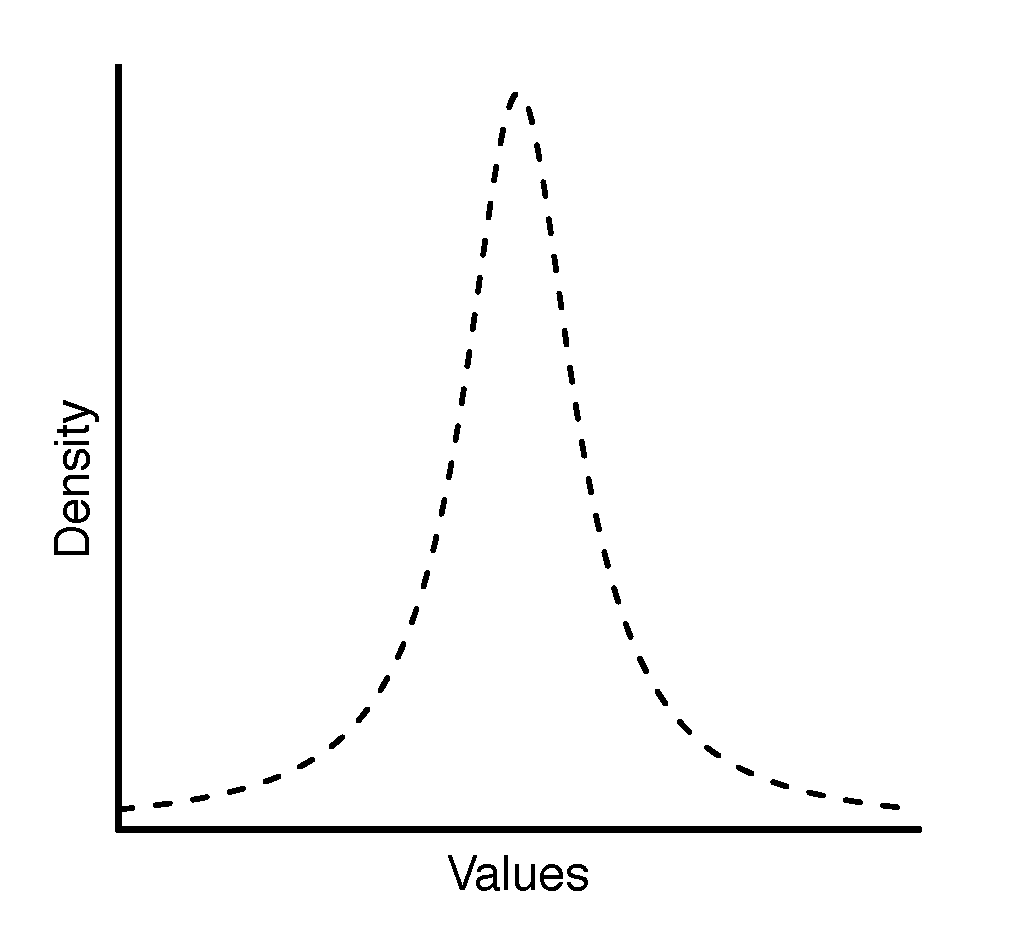
\includegraphics[width=0.32\textwidth]{./images/DensityCurves_student_t_mod.pdf}}&
\subfigure[Exponential]{\label{fig:density_exp}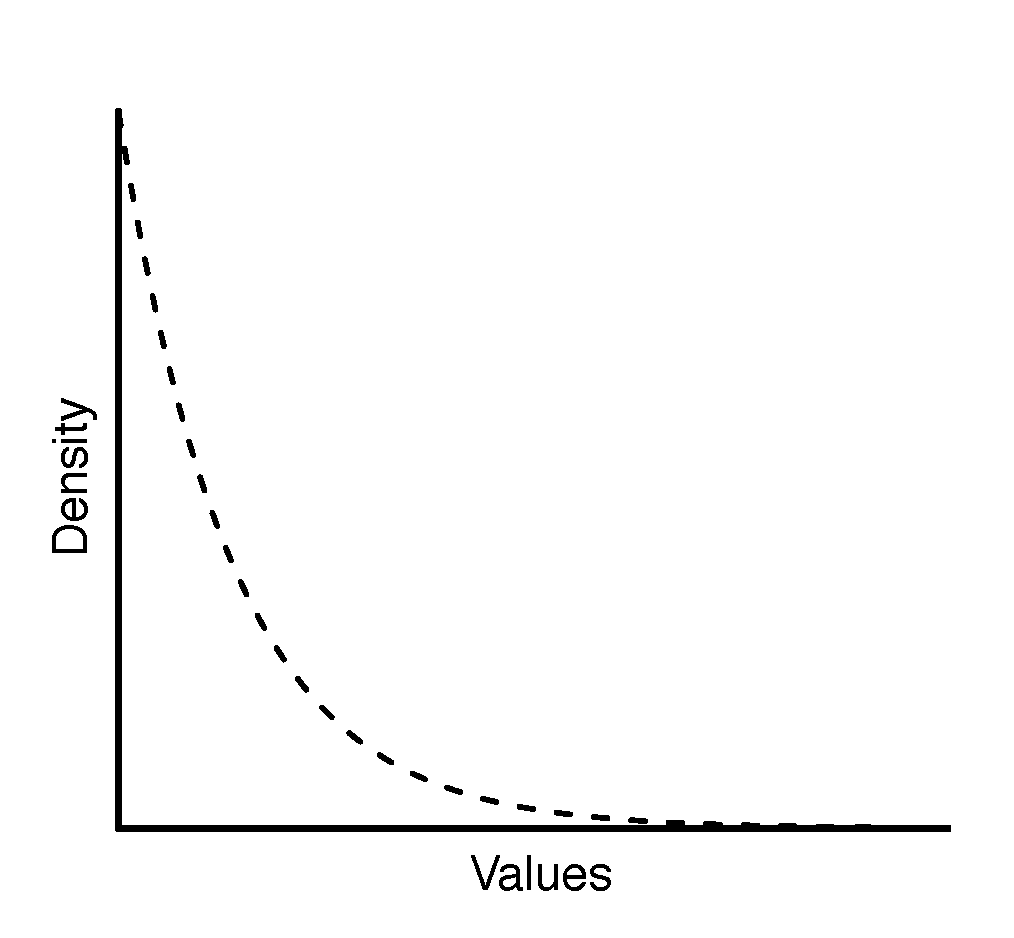
\includegraphics[width=0.32\textwidth]{./images/DensityCurves_exponential_mod.pdf}}&
\subfigure[Mixture of Gaussians]{\label{fig:density_multi}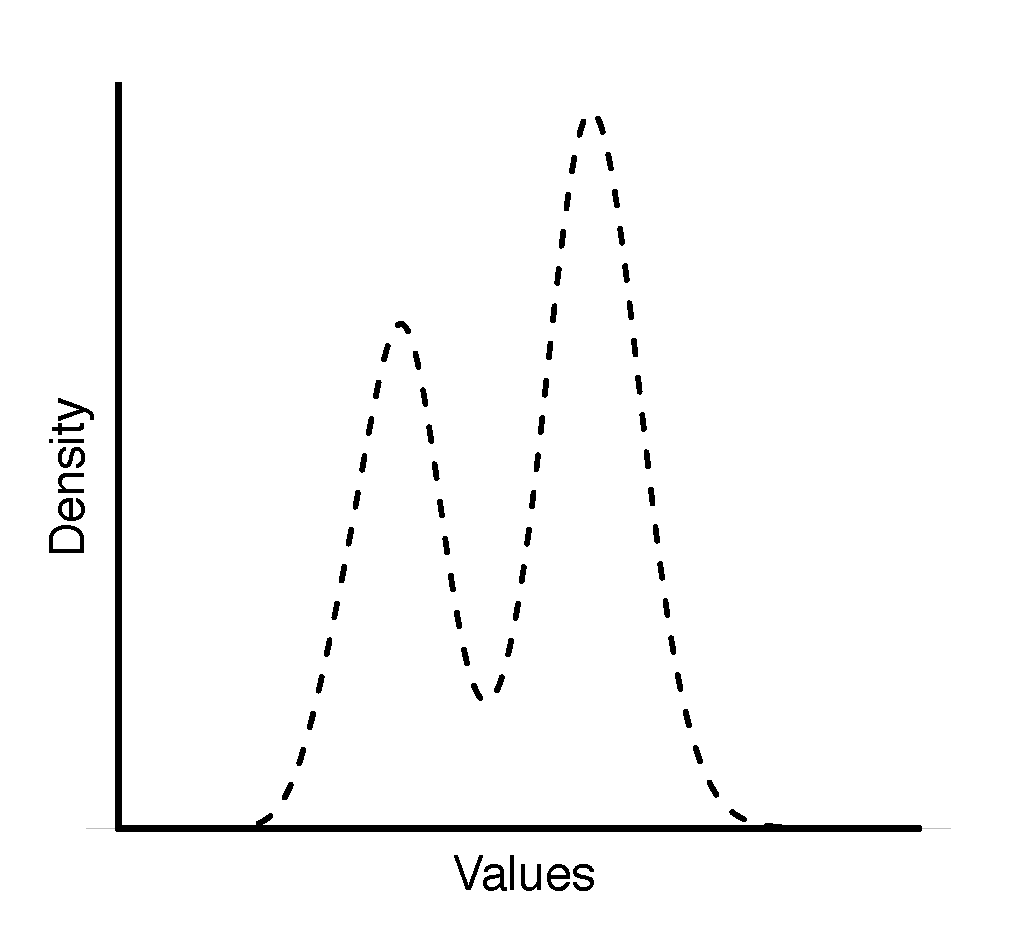
\includegraphics[width=0.32\textwidth]{./images/DensityCurves_mixture_of_gaussians_mod.pdf}}\\
\end{tabular}
\end{footnotesize}
\caption{Plots of some well known probability distributions.}
\label{fig:density_curves}
\end{figure}
\end{frame} 

 \begin{frame} 
\begin{figure}
\centerline{
\begin{tabular}{cc}
\subfigure[]{\label{fig:light_tails}\includegraphics[width=0.45\textwidth]{./images/pdf_HistogramFatLightTails_light.pdf}}&
\subfigure[]{\label{fig:fat_tails}\includegraphics[width=0.45\textwidth]{./images/pdf_HistogramFatLightTails_fat.pdf}}
\end{tabular}
}
\caption{Histograms of two unimodal datasets: (a) the distribution has light tails; (b) the distribution has fat tails.}
\label{fig:tails}
\end{figure}
\end{frame} 



 \begin{frame} 
\begin{figure}
\centerline{
\begin{tabular}{cc}
\subfigure[]{\label{fig:no_outliers}\includegraphics[width=0.45\textwidth]{./images/pdf_robust_studentt_nooutliers.pdf}}&
\subfigure[]{\label{fig:outliers}\includegraphics[width=0.45\textwidth]{./images/pdf_robust_studentt_outliers.pdf}}
\end{tabular}
}
\caption{Illustration of the robustness of the student-\textit{t} distribution to outliers: (a) a density histogram of a unimodal dataset overlaid with the density curves of a normal and a student-\textit{t} distribution that have been fitted to the data; (b) a density histogram of the same dataset with outliers added, overlaid with the density curves of a normal and a student-\textit{t} distribution that have been fitted to the data. The student-\textit{t} distribution is less affected by the introduction of outliers. (This figure is inspired by Figure 2.16 in (Bishop, 2006).)}
\label{fig:robustT}
\end{figure}
\end{frame} 


 \begin{frame} 
\begin{figure}
\centering
\begin{footnotesize}
\begin{tabular}{ccc}
\subfigure[]{\label{fig:mixed_gaussians}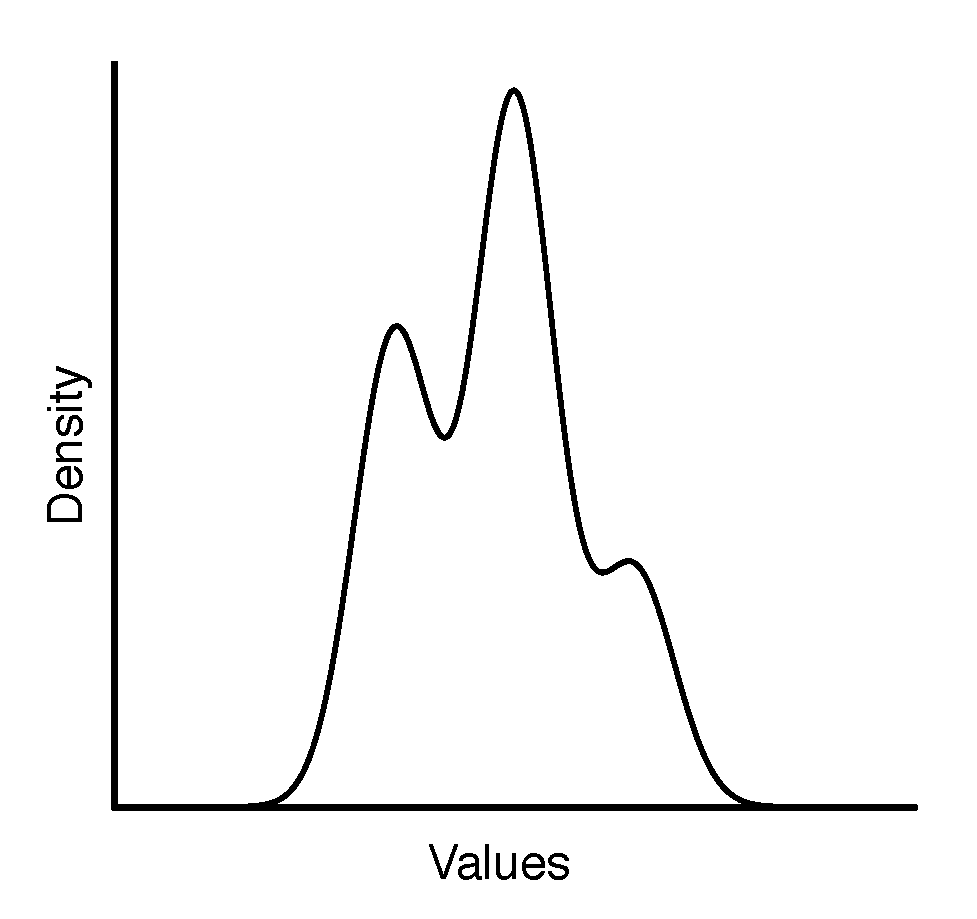
\includegraphics[width=0.32\textwidth]{./images/pdf_mixture_of_gaussians_1_mod.pdf}}&
\subfigure[]{\label{fig:separate_gaussians}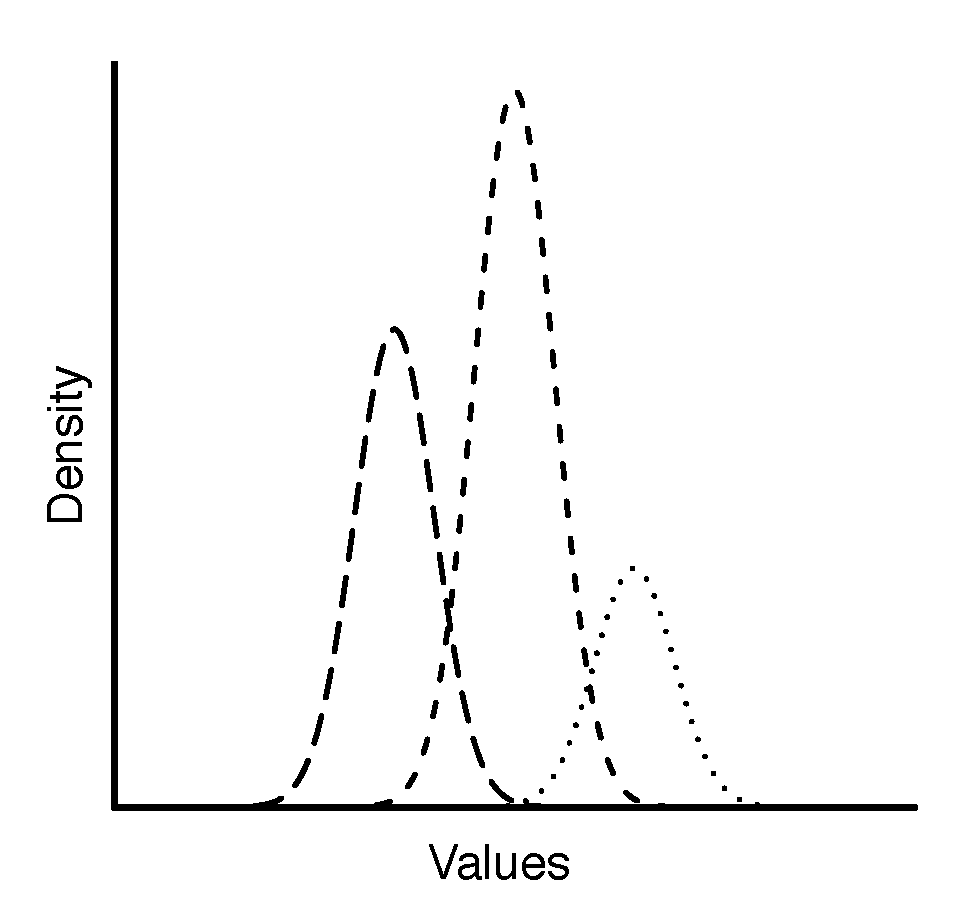
\includegraphics[width=0.32\textwidth]{./images/pdf_mixture_of_gaussians_2_mod.pdf}}&
\subfigure[]{\label{fig:mixed_gaussians_overlaid}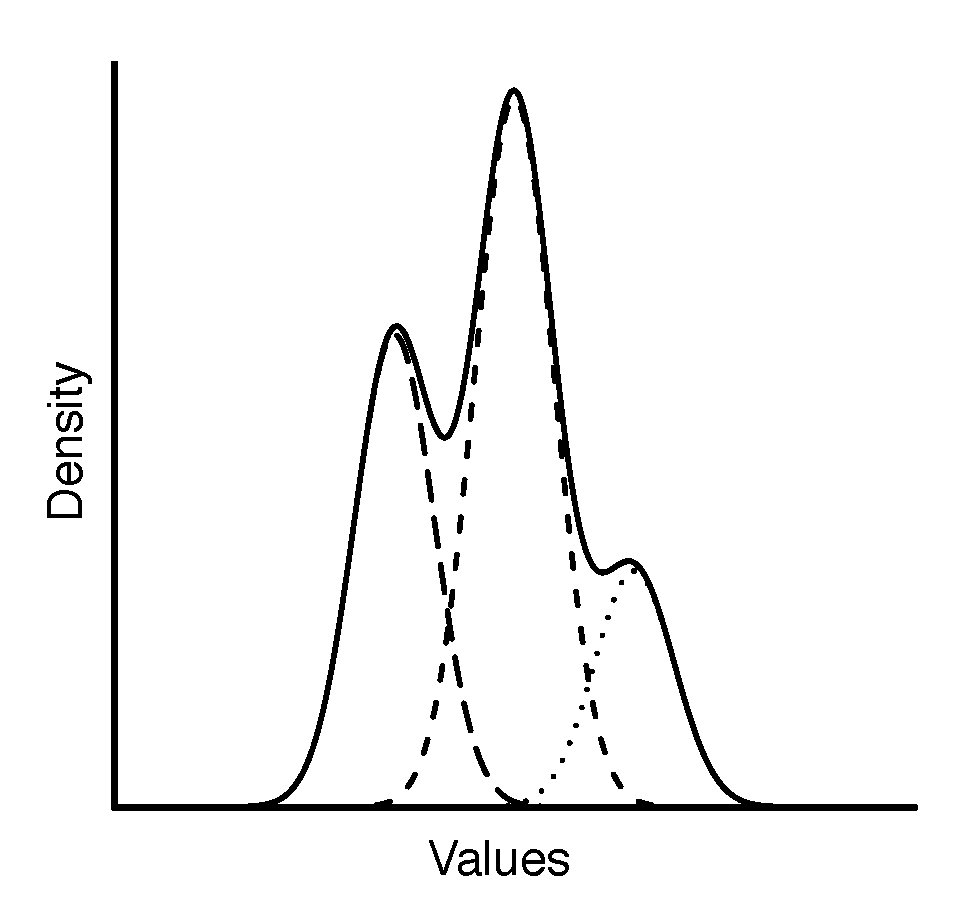
\includegraphics[width=0.32\textwidth]{./images/pdf_mixture_of_gaussians_3_mod.pdf}}\\
\end{tabular}
\end{footnotesize}
\caption{Illustration of how a mixture of Gaussians model is composed of a number of normal distributions. The curve plotted using a solid line is the mixture of Gaussians density curve, created using an appropriately weighted summation of the three normal curves, plotted using dashed and dotted lines.}
\label{fig:pdf_mixture_of_gaussians}
\end{figure}
\end{frame} 

\begin{frame} 
\begin{itemize}
\item A PDF is an abstraction over a density histogram and consequently PDF represents probabilities in terms of area under the curve. 
\item To use a PDF to calculate a probability we need to think in terms of the area under an interval of the PDF curve. 
\item We can calculate the area under a PDF by looking this up in a probability table or to use integration to calculate the area under the curve within the bounds of the interval.
\end{itemize}
\end{frame} 

 \begin{frame} 
\begin{figure}
\centering
\begin{footnotesize}
\begin{tabular}{ccc}
\subfigure[]{\label{fig:pdfapproxprob1}\includegraphics[width=0.32\textwidth]{./images/pdf_approx_prob_1.pdf}}&
\subfigure[]{\label{fig:pdfapproxprob2}\includegraphics[width=0.32\textwidth]{./images/pdf_approx_prob_2.pdf}}&
\subfigure[]{\label{fig:pdfapproxprob3}\includegraphics[width=0.32\textwidth]{./images/pdf_approx_prob_3.pdf}}\\
\end{tabular}
\end{footnotesize}
\caption{(a) The area under a density curve between the limits $x-\frac{\epsilon}{2}$ and $x+\frac{\epsilon}{2}$; (b) the approximation of this area computed by $PDF(x) \times \epsilon$; and (c) the error in the approximation is equal to the difference between area A, the area under the curve omitted from the approximation, and area B, the area above the curve erroneously included in the approximation. Both of these areas will get smaller as the width of the interval gets smaller, resulting in a smaller error in the approximation. }
\label{fig:pdfapproxprob}
\end{figure}
\end{frame} 

\begin{frame} 
\begin{itemize}
\item There is no hard and fast rule for deciding on \keyword{interval size} - instead, this decision is done on a case by case basis and is dependent on the precision required in answering a question. 
\item To illustrate how PDFs can be used in Naive Bayes models we will extend our loan application fraud detection query to have an \featN{Account Balance} feature
\end{itemize}
\end{frame} 


 \begin{frame} [plain]
\begin{table}[!tb]
\caption{The dataset from the loan application fraud detection domain with a new continuous descriptive features added: \featN{Account Balance}}
\label{table:fraudDetectionAccountBalanceLoanAmount}
\centering
\begin{tiny}
\resizebox{\textwidth}{!}{
\begin{tabular}{crrrrr}
\hline
~ & \featN{Credit} & \featN{Guarantor/} & ~ & \featN{Account} & ~\\
\featN{ID} & \featN{History} & \featN{CoApplicant} & \featN{Accommodation} & \featN{Balance} & \featN{Fraud}\\
\hline
1 & current  & none & 	own & $56.75$ &  true\\
2 & 	current & 	none & 	own & 	1,800.11 &false\\
3 & 	current & 	none & 	own & 	1,341.03 & false\\
4 & 	paid & 	guarantor & 	rent & 	$749.50$ &true\\
5 & 	arrears & 	none & 	own & 	1,150.00 &false\\
6 & 	arrears & 	none & 	own & 	$928.30$ &true\\
7 & 	current & 	none & 	own &  $250.90$& false\\
8 & 	arrears & 	none & 	own & 	$806.15$ &false\\
9 & 	current & 	none & 	rent & 1,209.02 &false\\
10 & 	none  & 	none & 	own& 	$405.72$ &true\\
11 & 	current & 	coapplicant & 	own & 	$550.00$ &false\\
12 & 	current & 	none & 	free & 	$223.89$ &true\\
13 & 	current & 	none & 	rent & 	$103.23$ &true\\
14 & 	paid & 	none & 	own & 	$758.22$ &false\\
15 & 	arrears & 	none & 	own & 	$430.79$ &false\\
16 & 	current & 	none & 	own & 	$675.11$  &false\\
17 & 	arrears & 	coapplicant & 	rent & 	1,657.20 &false\\
18 & 	arrears & 	none & 	free & 	1,405.18 &false\\
19 & 	arrears & 	none & 	own & 	$760.51$ &false\\
20 & 	current & 	none & 	own & $985.41$ &false\\
\hline
\end{tabular}
}
\end{tiny}
\end{table}
\end{frame} 

\begin{frame} 
\begin{itemize}
\item We need to define two PDFs for the new \featN{Account Balance} (AB) feature with each PDF conditioned on a different value in the domain or the target: 
\begin{itemize}
\item $P(AB=X|fr)=PDF_1(AB=X|fr)$ 
\item $P(AB=X|\lnot fr)=PDF_2(AB=X|\lnot fr)$
\end{itemize}
\item Note that these two PDFs do not have to be defined using the same statistical distribution. 
\end{itemize}
\end{frame} 

 \begin{frame} 
\begin{figure}
\centering
\begin{footnotesize}
\begin{tabular}{ccc}
\subfigure[]{\label{fig:fraud}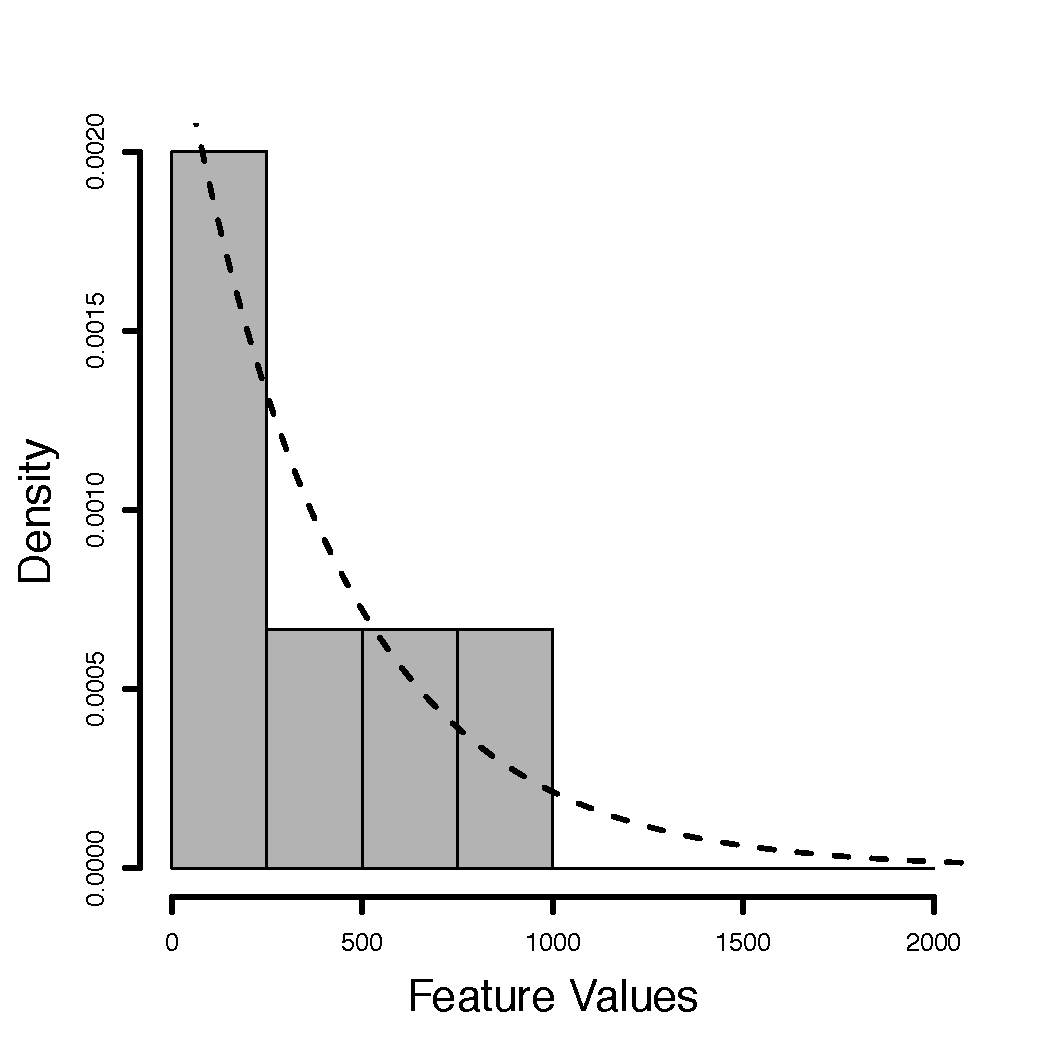
\includegraphics[width=0.45\textwidth]{./images/pdf_example_bank_balance_1_mod.pdf}}&
\subfigure[]{\label{fig:non_fraud}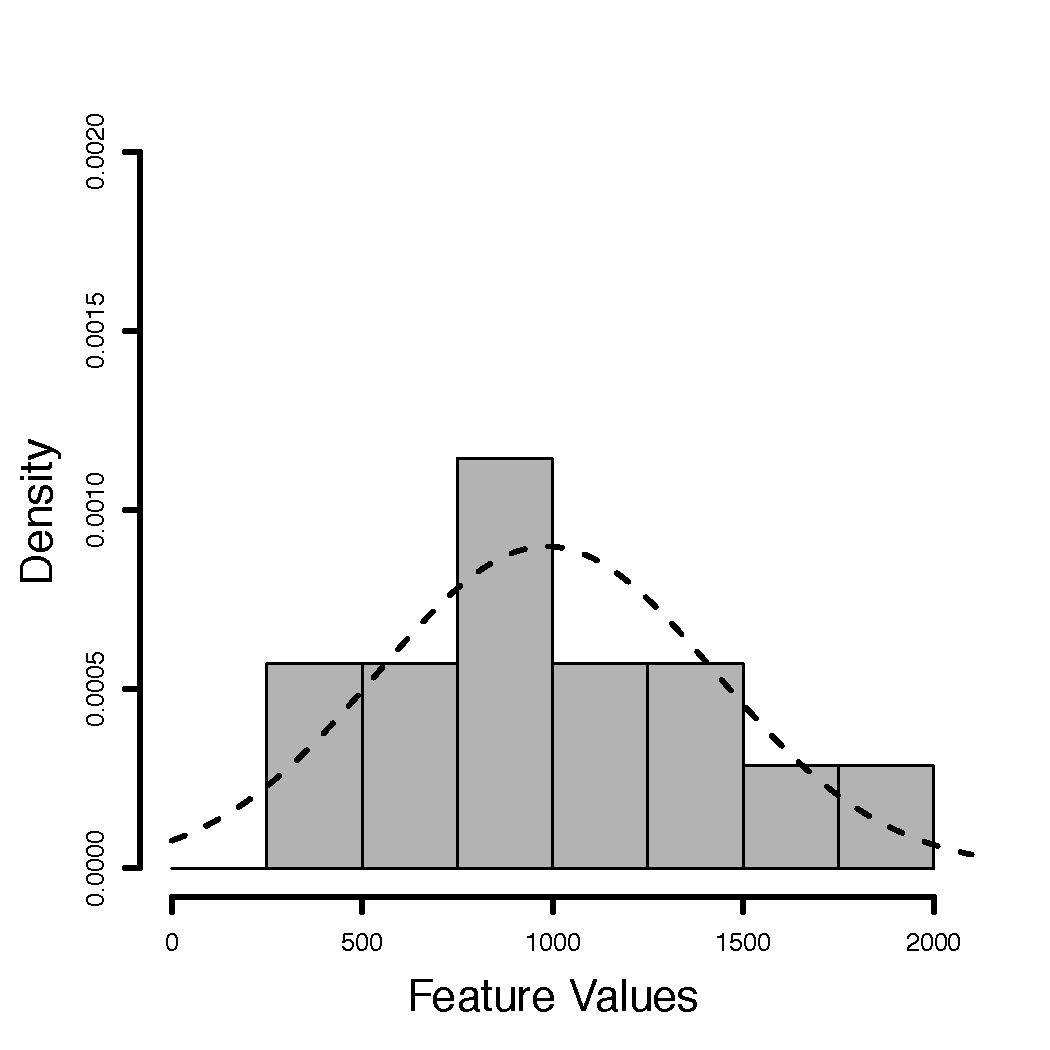
\includegraphics[width=0.45\textwidth]{./images/pdf_example_bank_balance_2_mod.pdf}}\\
\end{tabular}
\end{footnotesize}
\caption{Histograms, using a bin size of 250 units, and density curves for the \featN{Account Balance} feature: (a) the fraudulent instances overlaid with a fitted exponential distribution; (b) the non-fraudulent instances overlaid with a fitted normal distribution.}
\label{fig:pdf_fitting_distributions_bank_balance}
\end{figure}
\end{frame} 

\begin{frame} 
\begin{itemize}
\item From the shape of these histograms it appears that 
\begin{itemize}
\item the distribution of values taken by the \featN{Account Balance} feature in the set of instances where the target feature \featN{Fraudulent}=\featL{True} follows an exponential distribution
\item the distributions of values taken by the \featN{Account Balance} feature in the set of instances where the target feature \featN{Fraudulent}=\featL{False} is similar to a normal distribution. 
\end{itemize}
\item Once we have selected the distributions the next step is to fit the distributions to the data. 
\end{itemize}
\end{frame} 

\begin{frame} 
\begin{itemize}
\item To fit the exponential distribution we simply compute the sample mean, $\bar{x}$, of the \featN{Account Balance} feature in the set of instances where \featN{Fraudulent}=\featL{True} and set the $\lambda$ parameter equal to one divided by $\bar{x}$. 
\item To fit the normal distribution to the set of instances where \featN{Fraudulent}=\featL{False} we simply compute the sample mean and sample standard deviation, $s$, for the \featN{Account Balance} feature for this set of instances and set the parameters of the normal distribution to these values. 
\end{itemize}
\end{frame} 

 \begin{frame} [plain]
\begin{table}[!tb]
\caption{Partitioning the dataset based on the value of the target feature and fitting the parameters of a statistical distribution to model the \featN{Account Balance} feature in each partition.}
\label{table:exfittingdistributions}
\centering
\begin{footnotesize}
\begin{columns}
\begin{column}{0.5\textwidth}
\begin{tabular}{ccrr}
\hline
~ & ~ & \featN{Account} & ~\\
\featN{ID} & $\dots$ & \featN{Balance} & \featN{Fraud}\\
\hline
1 & ~ & $56.75$ & true\\
4 & 	~ & 	$749.50$ &true\\
6 & 	~ & 	$928.30$ &true\\
10 & 	$\dots$ & 	$405.72$ &true\\
12 & 	~ & 	$223.89$ &true\\
13 & 	~ & 	$103.23$ &true\\
\hline
\multicolumn{2}{l}{$\overline{\featN{AB}}$} & $411.22$ & ~\\
\multicolumn{2}{l}{$\lambda=^{1}!/_{\overline{\featN{AB}}}$} & $0.0024$ & ~ \\
\hline
\end{tabular}
\end{column} 
\begin{column}{0.5\textwidth}
\begin{tabular}{ccrr}
\hline
~ & ~ & \featN{Account} & ~\\
\featN{ID} & $\dots$ & \featN{Balance} & \featN{Fraud}\\
\hline
2 & 	~ & 	$1\,800.11$ &false\\
3 & 	~ & 	$1\,341.03$ &false\\
5 & 	~ & 	$1\,150.00$ &false\\
7 & 	~ & 	$250.90$ &false\\
8 & 	~ & 	$806.15$ &false\\
9 & 	~ & 	$1\,209.02$ &false\\
11 & 	~ & 	$550.00$ &false\\
14 & 	~ & 	$758.22$ &false\\
15 & 	~ & 	$430.79$ &false\\
16 & 	~ & 	$675.11$ &false\\
17 & 	~ & 	$1\,657.20$ &false\\
18 & 	~ & 	$1\,405.18$ &false\\
19 & 	~ & 	$760.51$ &false\\
20 & 	~ & 	$985.41$ &false\\
\hline
\multicolumn{2}{l}{$\overline{\featN{AB}}$} & $984.26$ & ~\\
\multicolumn{2}{l}{$sd(\featN{AB})$} & $460.94$ & ~\\
\hline
\end{tabular}
\end{column}
\end{columns}
\end{footnotesize}
\end{table}
\end{frame} 





 \begin{frame} 
\begin{table}
\caption{The Laplace smoothed (with $k=3$) probabilities needed by a naive Bayes prediction model calculated from the dataset in Table \ourRef{table:fraudDetectionAccountBalanceLoanAmount}, extended to include the conditional probabilities for the new \featN{Account Balance} feature, which are defined in terms of PDFs.}
\label{table:nbspdfs}
\begin{tiny}
\centerline{
	{\renewcommand{\arraystretch}{1.5}\begin{tabular}{ r c l r c l}
	\hline	
	$P(fr)$ & $=$ & $0.3$ & $P(\lnot fr)$ & $=$ & $0.7$\\
	$P(CH=none|fr)$ & $=$ & $0.2222$ & $P(CH=none|\lnot fr)$ & $=$ & $0.1154$\\
	$P(CH=paid|fr)$ & $=$ & $0.2222$ & $P(CH=paid|\lnot fr)$ & $=$ & $0.2692$\\
	$P(CH=current|fr)$ & $=$ & $0.3333$ & $P(CH=current|\lnot fr)$ & $=$ & $0.2692$\\
	$P(CH=arrears|fr)$ & $=$ & $0.2222$ & $P(CH=arrears|\lnot fr)$ & $=$ & $0.3462$\\
	$P(GC=none|fr)$ & $=$ & $0.5333$ & $P(GC=none|\lnot fr)$ & $=$ & $0.6522$\\
	$P(GC=guarantor|fr)$ & $=$ & $0.2667$ & $P(GC=guarantor|\lnot fr)$ & $=$ & $0.1304$\\
	$P(GC=coapplicant|fr)$ & $=$ & $0.2$ & $P(GC=coapplicant|\lnot fr)$ & $=$ & $0.2174$\\
	$P(ACC=own|fr)$ & $=$ & $0.4667$ & $P(ACC=own|\lnot fr)$ & $=$ & $0.6087$\\
	$P(ACC=rent|fr)$ & $=$ & $0.3333$ & $P(ACC=rent|\lnot fr)$ & $=$ & $0.2174$\\
	$P(ACC=free|fr)$ & $=$ & $0.2$ & $P(ACC=free|\lnot fr)$ & $=$ & $0.1739$\\
	$P(AB=x|fr)$ & ~ & ~ & $P(AB=x|\lnot fr)$ & ~ & ~\\
	$\approx$ 
& 
\multicolumn{2}{c}{$E\begin{pmatrix}x,\\\lambda=0.0024\end{pmatrix}$} 
& 
$\approx$ 
& 
\multicolumn{2}{c}{$N\begin{pmatrix}x,\\\mu =984.26,\\\sigma =460.94\end{pmatrix}$} 
\\
	\hline
	\end{tabular}}
}
\end{tiny}
\end{table}
\end{frame} 

 \begin{frame} 
\begin{table}[!tb]
\caption{A query loan application from the fraud detection domain.}
\label{table:fraudDetectionQueryPDF}
\centering
\begin{footnotesize}
\resizebox{\textwidth}{!}{\begin{tabular}{rrrrr}
\hline
\textbf{Credit} & \textbf{Guarantor/} & ~ & \textbf{Account} & ~\\
\textbf{History} & \textbf{CoApplicant} & \textbf{Accomodation} & \textbf{Balance} & \textbf{Fraudulent}\\
\hline
paid & guarantor & free & $759.07$ &?\\
\hline
\end{tabular}}
\end{footnotesize}
\end{table}
\end{frame} 


 \begin{frame} 
\begin{table}
\caption{The probabilities, from Table \ourRef{table:nbspdfs}, needed by the naive Bayes prediction model to make a prediction for the query $\left<\featN{CH} = \featL{paid}, \featN{GC} = \featL{guarantor}, \featN{ACC} = \featL{free}, \featN{AB}=759.07\right>$ and the calculation of the scores for each candidate prediction.}
\label{table:nbexcalculationsPDF}
\begin{footnotesize}
\centerline{
	{\renewcommand{\arraystretch}{1.5}\begin{tabular}{r c l r c l}
	\hline
	$P(fr)$ & $=$ & $0.3$ & $P(\lnot fr)$ & $=$ & $0.7$\\
	$P(CH=paid|fr)$ & $=$ & $0.2222$ & $P(CH=paid|\lnot fr)$ & $=$ & $0.2692$\\
	$P(GC=guarantor|fr)$ & $=$ & $0.2667$ & $P(GC=guarantor|\lnot fr)$ & $=$ & $0.1304$\\
	$P(ACC=free|fr)$ & $=$ & $0.2$ & $P(ACC=free|\lnot fr)$ & $=$ & $0.1739$\\
	$P(AB=759.07|fr)$ & $~$ & ~ & $P(AB=759.07|\lnot fr)$ & $~$\\
	$\approx E\begin{pmatrix}759.07,\\\lambda=0.0024\end{pmatrix}$ & $=$ & $0.00039$ & $\approx N\begin{pmatrix}759.07,\\\mu =984.26,\\\sigma =460.94\end{pmatrix}$ & $=$ & $0.00077$\\
	\hline
      \multicolumn{4}{c}{$\left( \prod_{k=1}^m P(\mathbf{q}[k]|fr) \right) \times P(fr) =0.0000014$}\\
 	\multicolumn{4}{c}{$\left( \prod_{k=1}^m P(\mathbf{q}[k]|\lnot fr) \right) \times P(\lnot fr) = 0.0000033$}\\
	\hline
	\end{tabular}}
}
\end{footnotesize}
\end{table}
\end{frame} 


\SectionSlideShortHeader{Continuous Features: Binning}{Binning}

\begin{frame} 
\begin{itemize}
\item In Section 3.6.2 we explained two of the best known binning techniques  \keyword{equal-width} and \keyword{equal-frequency}.
\item We can use these techniques to \textit{bin} continuous features into categorical features
\item In general we recommend \keyword{equal-frequency binning}.
\end{itemize}
\end{frame} 

 \begin{frame} [plain]
\begin{table}[!tb]
\caption{The dataset from a loan application fraud detection domain with a second continuous descriptive feature added: \featN{Loan Amount}}
\label{table:fraudDetectionLoanAmount}
\centering
\begin{footnotesize}
\resizebox{\textwidth}{!}{
\begin{tabular}{crrrrrr}
\hline
~ & \featN{Credit} & \featN{Guarantor/} & ~ & \featN{Account} & \featN{Loan} & ~\\
\featN{ID} & \featN{History} & \featN{CoApplicant} & \featN{Accommodation} & \featN{Balance} & \featN{Amount} & \featN{Fraud}\\
\hline
1 & current  & none & 	own & $56.75$ & 900 & true\\
2 & 	current & 	none & 	own & 	1\,800.11& 	150\,000 &false\\
3 & 	current & 	none & 	own & 	1\,341.03 & 	48\,000& false\\
4 & 	paid & 	guarantor & 	rent & 	$749.50$ & 	10\,000&true\\
5 & 	arrears & 	none & 	own & 	1\,150.00 & 	32\,000&false\\
6 & 	arrears & 	none & 	own & 	$928.30$ & 	250\,000&true\\
7 & 	current & 	none & 	own &  $250.90$& 	25\,000& false\\
8 & 	arrears & 	none & 	own & 	$806.15$ & 	18\,500&false\\
9 & 	current & 	none & 	rent & 1\,209.02 & 	20\,000&false\\
10 & 	none  & 	none & 	own& 	$405.72$ & 	9\,500&true\\
11 & 	current & 	coapplicant & 	own & 	$550.00$ & 	16\,750&false\\
12 & 	current & 	none & 	free & 	$223.89$ & 	9\,850&true\\
13 & 	current & 	none & 	rent & 	$103.23$ & 	95\,500&true\\
14 & 	paid & 	none & 	own & 	$758.22$ & 	65\,000&false\\
15 & 	arrears & 	none & 	own & 	$430.79$ & 	500&false\\
16 & 	current & 	none & 	own & 	$675.11$  & 	16\,000&false\\
17 & 	arrears & 	coapplicant & 	rent & 	1\,657.20 & 	15\,450&false\\
18 & 	arrears & 	none & 	free & 	1\,405.18 & 	50\,000&false\\
19 & 	arrears & 	none & 	own & 	$760.51$ & 	500&false\\
20 & 	current & 	none & 	own & $985.41$ & 	35\,000&false\\
\hline
\end{tabular}
}
\end{footnotesize}
\end{table}
\end{frame} 

 \begin{frame} [plain]
\begin{table}[htb]
\caption{The \featN{Loan Amount} continuous feature discretized into 4 equal-frequency bins.}
\label{tab:equalfrequencybinning}
\centering
\begin{tiny}
\begin{tabular}{cc}
		\hline
			\begin{minipage}{0.46\textwidth}
\begin{tabular}{crrc}
~ & \featN{} & \featN{Binned} & ~\\
~ & \featN{Loan} & \featN{Loan} & ~\\
\featN{ID} & \featN{Amount} & \featN{Amount} & \featN{Fraud}\\
\hline
15 & 	500 & 	bin1 &false\\
19 & 	500 & 	bin1 &false\\
1 & 900 & bin1 & true\\
10 & 	9,500 & 	bin1 &true\\
12 & 	9,850 & 	bin1 &true\\
4 & 	10,000 & 	bin2 &true\\
17 & 	15,450 & 	bin2 &false\\
16 & 	16,000 & 	bin2 &false\\
11 & 	16,750 & 	bin2 &false\\
8 & 	18,500 & 	bin2 &false\\
\hline
\end{tabular}
\end{minipage}
\begin{minipage}{0.46\textwidth}
\begin{tabular}{crrc}
~ & \featN{} & \featN{Binned} & ~\\
~ & \featN{Loan} & \featN{Loan} & ~\\
\featN{ID} & \featN{Amount} & \featN{Amount} & \featN{Fraud}\\
\hline
9 & 	20,000 & 	bin3 &false\\
7 & 	25,000 & 	bin3 &false\\
5 & 	32,000 & 	bin3 &false\\
20 & 	35,000 & 	bin3 &false\\
3 & 	48,000 & 	bin3 &false\\
18 & 	50,000 & 	bin4 &false\\
14 & 	65,000 & 	bin4 &false\\
13 & 	95,500 & 	bin4 &true\\
2 & 	150,000 & 	bin4 &false\\
6 & 	250,000 & 	bin4 &true\\
\hline
\end{tabular}
\end{minipage}
\end{tabular}
\end{tiny}
\end{table}
\end{frame} 

\begin{frame} 
\begin{itemize}
\item Once we have discretized the data we need to record the raw continuous feature threshold between the bins so that we can use these for query feature values. 
\end{itemize}
\begin{table}[!tb]
\caption{The thresholds used to discretize the \featN{Loan Amount} feature in queries.}
\label{table:binthresholds}
\centering
\begin{footnotesize}
\begin{tabular}{ rcl }
\hline
\multicolumn{3}{c}{\textbf{Bin Thresholds}}\\
\hline
~ &  Bin1 & $\leq 9,925$\\
$9,925<$ &  Bin2 & $\leq 19,250$\\
$19,225<$ &  Bin3 & $\leq 49,000$\\
$49,000<$ &  Bin4 & ~\\
\hline
\end{tabular}
\end{footnotesize}
\end{table}
\end{frame} 

 \begin{frame} [plain]
\begin{table}
\caption{The Laplace smoothed (with $k=3$) probabilities needed by a naive Bayes prediction model calculated from the fraud detection dataset. Notation key: FR = \featN{Fraud}, CH = \featN{Credit History}, AB = \featN{Account Balance}, GC = \featN{Guarantor/CoApplicant}, ACC = \featN{Accommodation}, BLA = \featN{Binned Loan Amount}.}
\label{table:nbsmoothedwithdiscretized}
\begin{tiny}
\centerline{
	{\renewcommand{\arraystretch}{1.4}\begin{tabular}{ r c l r c l}
	\hline
	$P(fr)$ & $=$ & $0.3$ & $P(\lnot fr)$ & $=$ & $0.7$\\
	$P(CH=none|fr)$ & $=$ & $0.2222$ & $P(CH=none|\lnot fr)$ & $=$ & $0.1154$\\
	$P(CH=paid|fr)$ & $=$ & $0.2222$ & $P(CH=paid|\lnot fr)$ & $=$ & $0.2692$\\
	$P(CH=current|fr)$ & $=$ & $0.3333$ & $P(CH=current|\lnot fr)$ & $=$ & $0.2692$\\
	$P(CH=arrears|fr)$ & $=$ & $0.2222$ & $P(CH=arrears|\lnot fr)$ & $=$ & $0.3462$\\
	$P(GC=none|fr)$ & $=$ & $0.5333$ & $P(GC=none|\lnot fr)$ & $=$ & $0.6522$\\
	$P(GC=guarantor|fr)$ & $=$ & $0.2667$ & $P(GC=guarantor|\lnot fr)$ & $=$ & $0.1304$\\
	$P(GC=coapplicant|fr)$ & $=$ & $0.2$ & $P(GC=coapplicant|\lnot fr)$ & $=$ & $0.2174$\\
	$P(ACC=own|fr)$ & $=$ & $0.4667$ & $P(ACC=own|\lnot fr)$ & $=$ & $0.6087$\\
	$P(ACC=rent|fr)$ & $=$ & $0.3333$ & $P(ACC=rent|\lnot fr)$ & $=$ & $0.2174$\\
	$P(ACC=free|fr)$ & $=$ & $0.2$ & $P(ACC=free|\lnot fr)$ & $=$ & $0.1739$\\
	$P(AB=x|fr)$ & $~$ & $~$ & $P(AB=x|\lnot fr)$ & $~$ & $~$\\
	\multicolumn{3}{c}{$\approx~E\begin{pmatrix}x,\\\lambda=0.0024\end{pmatrix}$} & 	 	\multicolumn{3}{c}{$\approx~N\begin{pmatrix}x,\\\mu =984.26,\\\sigma =460.94\end{pmatrix}$}\\
	$P(BLA=bin1|fr)$ & $=$ & $0.3333$ & $P(BLA=bin1|\lnot fr)$ & $=$ & $0.1923$\\
	$P(BLA=bin2|fr)$ & $=$ & $0.2222$ & $P(BLA=bin2|\lnot fr)$ & $=$ & $0.2692$\\
	$P(BLA=bin3|fr)$ & $=$ & $0.1667$ & $P(BLA=bin3|\lnot fr)$ & $=$ & $0.3077$\\
	$P(BLA=bin4|fr)$ & $=$ & $0.2778$ & $P(BLA=bin4|\lnot fr)$ & $=$ & $0.2308$\\
	\hline
	\end{tabular}}
}
\end{tiny}
\end{table}
\end{frame} 

 \begin{frame} 
\begin{table}[!tb]
\caption{A query loan application from the fraud detection domain.}
\label{table:fraudDetectionQuery4}
\centering
\begin{footnotesize}
\resizebox{\textwidth}{!}{\begin{tabular}{rrrrrr}
\hline
\textbf{Credit} & \textbf{Guarantor/} & ~ & \textbf{Account} &\textbf{Loan} & ~\\
\textbf{History} & \textbf{CoApplicant} & \textbf{Accomodation} & \textbf{Balance} & \textbf{Amount} & \textbf{Fraudulent}\\
\hline
paid & guarantor & free & $759.07$ & 8,000 &?\\
\hline
\end{tabular}}
\end{footnotesize}
\end{table}
\end{frame} 

 \begin{frame} [plain]
\begin{table}
\caption{The relevant smoothed probabilities, from Table \ourRef{table:nbsmoothedwithdiscretized}, needed by the naive Bayes model to make a prediction for the query $\left<\featN{CH} = \featL{paid}, \featN{GC} = \featL{guarantor}, \featN{ACC} = \featL{free}, \featN{AB}=759.07, \featN{LA}=8\,000\right>$ and the calculation of the scores for each candidate prediction.}
\label{table:nbexcalculations4}
	\centering
\begin{footnotesize}
\centerline{
	{\renewcommand{\arraystretch}{1.5}\begin{tabular}{ r c l r c l}
	\hline
	$P(fr)$ & $=$ & $0.3$ & $P(\lnot fr)$ & $=$ & $0.7$\\
	$P(CH=paid|fr)$ & $=$ & $0.2222$ & $P(CH=paid|\lnot fr)$ & $=$ & $0.2692$\\
	$P(GC=guarantor|fr)$ & $=$ & $0.2667$ & $P(GC=guarantor|\lnot fr)$ & $=$ & $0.1304$\\
	$P(ACC=free|fr)$ & $=$ & $0.2$ & $P(ACC=free|\lnot fr)$ & $=$ & $0.1739$\\
	$P(AB=759.07|fr)$ & $~$ & ~ & $P(AB=759.07|\lnot fr)$ & $~$ & $~$\\
	$\approx~E\begin{pmatrix}759.07,\\\lambda=0.0024\end{pmatrix}$ & $=$ & $0.00039$ & $\approx~N\begin{pmatrix}759.07,\\\mu =984.26,\\\sigma =460.94\end{pmatrix}$ & $=$ & $0.00077$\\
	$P(BLA=bin1|fr)$ & $=$ & $0.3333$ & $P(BLA=bin1|\lnot fr)$ & $=$ & $0.1923$\\
	\hline
      \multicolumn{6}{c}{$\left( \prod_{k=1}^m P(\mathbf{q}[k] \mid fr) \right) \times P(fr) =0.000000462$}\\
 	\multicolumn{6}{c}{$\left( \prod_{k=1}^n P(\mathbf{q}[k] \mid \lnot fr) \right) \times P(\lnot fr) =0.000000633$}\\
	\hline
	\end{tabular}}
}
\end{footnotesize}
\end{table}
\end{frame} 



\SectionSlideShortHeader{Bayesian Networks}{Bayesian Nets}

\begin{frame}
	\begin{itemize}
		\item \keyword{Bayesian networks} use a graph-based representation to encode the structural relationships---such as direct influence and conditional independence---between subsets of features in a domain.
		\item Consequently, a Bayesian network representation is generally more compact than a full joint distribution, yet is not forced to assert global conditional independence between all descriptive features.
	\end{itemize}
\end{frame}

\begin{frame}
A Bayesian Network is a directed acyclical graph that is composed of thee basic elements:
\begin{itemize}
	\item nodes
	\item edges
	\item conditional probability tables (CPT)
\end{itemize}
\end{frame}

 \begin{frame} 
\begin{figure}
\centering
\begin{tabular}{cc}
\subfigure[]{\label{fig:bn1}\includegraphics[width=0.35\textwidth]{./images/bn1.pdf}} &
\subfigure[]{\label{fig:bn1Cseq}\includegraphics[width=0.4\textwidth]{./images/bn1CseqParents.pdf}}\\
\end{tabular}
\caption{(a) A Bayesian network for a domain consisting of two binary features. The structure of the network states that the value of feature A directly influences the value of feature B. (b) A Bayesian network consisting of 4 binary features with a path containing 3 generations of nodes: D, C, and B.}
\label{fig:bnssidebyside}
\end{figure}
\end{frame} 

 \begin{frame} 
 \begin{itemize}
 	\item In probability terms the directed edge from A to B in Figure (a) on the previous slide states that:
\end{itemize}
\begin{equation}
P(A,B)=P(B|A) \times P(A)
\label{bn:edgesemantics}
\end{equation}
\begin{itemize}
	\item For example, the probability of the event $a$ and $\lnot b$ is
\end{itemize}
\begin{equation*}
P(a,\lnot b)=P(\lnot b|a) \times P(a) = 0.7 \times 0.4 = 0.28
\end{equation*}
\end{frame} 

 \begin{frame} 
 \begin{itemize}
 	\item Equation \ourEqRef{bn:edgesemantics} can be generalized to the statement that for any network with $N$ nodes, the probability of an event $x_1, \dots, x_n$,  can be computed using the following formula:
\end{itemize}
\begin{equation}
P(x_1, \dots, x_n ) = \prod_{i=1}^n P(x_i|Parents(x_i))
\label{eq:bnparents}
\end{equation}
\end{frame} 



 \begin{frame} 
 \begin{itemize}
 	\item For example, using the more complex Bayesian network in figure (b) above, we can calculate the probability of the joint event $P(a, \lnot b, \lnot c, d)$ as follows:
\end{itemize}
\begin{align*}
P(a, \lnot b, \lnot c, d) &= P(\lnot b | a, \lnot c) \times P(\lnot c | d) \times P(a) \times P(d)\\
&= 0.5 \times 0.8 \times 0.4 \times 0.4 = 0.064
\end{align*}
\end{frame} 

 \begin{frame} 
 \begin{itemize}
 	\item We can uses Bayes' Theorem to invert the dependencies between nodes in a network.
	\item Returning to the simpler network in figure (a) above we can calculate $P(a|\lnot b)$ as follows:
\end{itemize}
\begin{align*}
P(a|\lnot b) &= \frac{P(\lnot b | a) \times P(a)}{P(\lnot b)} = \frac{P(\lnot b | a) \times P(a)}{\sum_i P(\lnot b|A_i)}\\
&= \frac{P(\lnot b | a) \times P(a)}{\left(P(\lnot b|a)\times P(a)\right) + \left(P(\lnot b|\lnot a)\times P(\lnot a)\right)}\\
&= \frac{0.7 \times 0.4}{\left(0.7\times 0.4\right) + \left(0.6\times 0.6\right)}=0.4375\\
\end{align*}
\end{frame} 

\begin{frame}
	\begin{itemize}
		\item For conditional independence we need to take into account not only the parents of a node by also the state of its children and their parents.
		\item The set of nodes in a graph that make a node independent of the rest of the graph are known as the \keyword{Markov blanket} of a node.
	\end{itemize}
\end{frame}

 \begin{frame} 
\begin{figure}
\centering
\includegraphics[width=0.25\textwidth]{./images/markovblanket.pdf}\\
\caption{A depiction of the Markov blanket of a node. The gray nodes define the Markov blanket of the black node. The black node is conditionally independent of the white nodes given the state of the gray nodes.}
\label{fig:markovblanket}
\end{figure}
\end{frame} 



 \begin{frame} 
 \begin{itemize}
 	\item The conditional independence of a node $x_i$ in a graph with $n$ nodes is defines as:
\end{itemize}
\begin{alignat}{2}
P(x_i&| x_1, \dots, x_{i-1}, x_{i+1}, \dots, x_n) = \notag\\
 &P(x_i|Parents(x_i)) \prod_{j \in Children(x_i)} P(x_j|Parents(x_j))
\label{eq:bnconditional}
\end{alignat}
\end{frame} 



 \begin{frame} 
 \begin{itemize}
 	\item Applying the equation of the preceding slide to the network in figure (b) above we can calculate the probability of $P(c|\lnot a, b , d)$ as
\end{itemize}

\begin{align*}
P(c|\lnot a, b , d) &= P(c|d) \times P(b|c,\lnot a)\\
&= 0.2 \times 0.4 = 0.08
\end{align*}
\end{frame} 

\begin{frame}
 \begin{itemize}
 	\item A naive Bayes classifier is a Bayesian network with a specific topological structure.
\end{itemize}
\end{frame}

 \begin{frame} 
\begin{figure}
\centering
\begin{footnotesize}
\begin{tabular}{cc}
\subfigure[]{\label{fig:nbbn}\includegraphics[width=0.4\textwidth]{./images/nbbn.pdf}} &
\subfigure[]{\label{fig:fraudbn}\includegraphics[width=0.6\textwidth]{./images/fraudnbbn.pdf}}\\
\end{tabular}
\end{footnotesize}
\caption{(a) A Bayesian network representation of the conditional independence asserted by a naive Bayes model between the descriptive features given knowledge of the target feature; (b) a Bayesian network representation of the conditional independence assumption for the naive Bayes model in the fraud example.}
\label{fig:nbbnstruct}
\end{figure}
\end{frame} 



 \begin{frame} 
  \begin{itemize}
 	\item When we computed a conditional probability for a target feature using a naive Bayes model, we used the following calculation
\end{itemize}
\begin{equation*}
P(t| \mathbf{d}[1], \dots,\mathbf{d}[n]) = P(t) \prod_{j \in Children(t)} P(\mathbf{d}[j]|t)
\end{equation*}
  \begin{itemize}
 	\item This equation is equivalent to Equation \ourEqRef{eq:bnconditional} from earlier.
\end{itemize}

\end{frame} 

\begin{frame}
	\begin{itemize}
			\item Computing a conditional probability for a node becomes more complex if the value of one or more of the parent nodes is unknown.
	\end{itemize}
\end{frame}

 \begin{frame} 
 \begin{itemize}
 	\item For example, in the context of the network in figure (b) above, to compute $P(b|a, d)$ where the status of node $C$ in unknown we would do the following calculations:
\end{itemize}
\begin{enumerate}
	\item Compute the distribution for $C$ given $D$: $P(c\mid d)=0.2$,  $P(\lnot c\mid d)=0.8$
	\item Compute $P(b\mid a,C)$ by summing out $C$: $P(b\mid a,C)=\sum_i P(b\mid a,C_i)$
\begin{footnotesize}
\begin{align*}
P(b\mid a, C) &= \sum_i P(b\mid a,C_i) =\sum_i \frac{P(b,a,C_i)}{P(a,C_i)}\\
&= \frac{(P(b\mid a,c) \times P(a) \times P(c))+(P(b\mid a,\lnot c) \times P(a) \times P(\lnot c))}{(P(a)\times P(c))+(P(a)\times P(\lnot c))}\\
&= \frac{(0.2 \times 0.4 \times 0.2)+ (0.5 \times 0.4 \times 0.8)}{(0.4\times0.2)+(0.4\times0.8)} = 0.44
\end{align*}
\end{footnotesize}
\end{enumerate}
\end{frame}

\begin{frame}
	\begin{itemize}
		\item  This example illustrates the power of Bayesian networks. 
		\begin{itemize}
			\item When complete knowledge of the state of all the nodes in the network is not available, we clamp the values of nodes that we do have knowledge of and sum out the unknown nodes. 
		\end{itemize}
	\end{itemize}
\end{frame} 

 \begin{frame} 
\begin{figure}
\centering
\begin{footnotesize}
\begin{tabular}{cc}
\subfigure[]{\label{fig:bn2}\includegraphics[width=0.3\textwidth]{./images/bn2.pdf}} &
\subfigure[]{\label{fig:bn3}\includegraphics[width=0.3\textwidth]{./images/bn3.pdf}} \\
\end{tabular}
\end{footnotesize}
\caption{Two different Bayesian networks, each defining the same full joint probability distribution.}
\label{fig:bnmultiple}
\end{figure}
\end{frame} 



 \begin{frame} 
\begin{itemize}
	\item We can illustrate that these two networks encode the same joint probability distribution by using each network to compute $P(\lnot a,b,c)$
	\item Using network (a) we get:
\begin{alignat*}{2}
P(&\lnot a,b,c)=P(c|\lnot a,b) \times P(b|\lnot a) \times P(\lnot a)\\
&= 0.25 \times 0.5 \times 0.4 = 0.05
\end{alignat*}
	\item Using network (b) we get:
\begin{alignat*}{2}
P(&\lnot a,b,c)=P(\lnot a|c,b) \times P(b|c) \times P(c)\\
& = 0.5 \times 0.5 \times 0.2 = 0.05
\end{alignat*}
\end{itemize}
\end{frame} 

\begin{frame}
	\begin{itemize}
		\item The simplest was to construct a Bayesian network is to use a hybrid approach where:
		\begin{enumerate}
			\item the topology of the network is given to the learning algorithm,
			\item and the learning task involves inducing the CPT from the data.
		\end{enumerate}
	\end{itemize}
\end{frame}

 \begin{frame} 
\begin{table}[htb]
	\caption{(a) Some socio-economic data for a set of countries; (b) a binned version of the data listed in (a).}
	\label{tab:corrdata}
\begin{tiny}
		\begin{tabular}{l|rrrr|rrrr}
\hline		
\featN{Country} & \featN{Gini} & \featN{School} & \featN{Life} & ~ & \featN{Gini} & \featN{School} & \featN{Life} & ~\\
\featN{ID} & \featN{Coef} & \featN{Years} & \featN{Exp} & \featN{CPI} &\featN{Coef} & \featN{Years} & \featN{Exp} & \featN{CPI}\\
\hline
Afghanistan & 27.82 & 0.40 & 59.61 & 1.52 & low & low & low & low\\
Argentina & 44.49 & 10.10 & 75.77 & 3.00 & high & low & low & low\\
Australia & 35.19 & 11.50 & 82.09 & 8.84 & low & high & high & high\\
Brazil & 54.69 & 7.20 & 73.12 & 3.77 & high & low & low & low\\
Canada & 32.56 & 14.20 & 80.99 & 8.67 & low & high & high & high\\
China & 42.06 & 6.40 & 74.87 & 3.64 & high & low & low & low\\
Egypt & 30.77 & 5.30 & 70.48 & 2.86 & low & low & low & low\\
Germany & 28.31 & 12.00 & 80.24 & 8.05 & low & high & high & high\\
Haiti & 59.21 & 3.40 & 45.00 & 1.80 & high & low & low & low\\
Ireland & 34.28 & 11.50 & 80.15 & 7.54 & low & high & high & high\\
Israel & 39.2 & 12.50 & 81.30 & 5.81 & low & high & high & high\\
New Zealand & 36.17 & 12.30 & 80.67 & 9.46 & low & high & high & high\\
Nigeria & 48.83 & 4.10 & 51.30 & 2.45 & high & low & low & low\\
Russia & 40.11 & 12.90 & 67.62 & 2.45 & high & high & low & low\\
Singapore & 42.48 & 6.10 & 81.788 & 9.17 & high & low & high & high\\
South Africa & 63.14 & 8.50 & 54.547 & 4.08 & high & low & low & low\\
Sweden & 25.00 & 12.80 & 81.43 & 9.30 & low & high & high & high\\
U.K. & 35.97 & 13.00 & 80.09 & 7.78 & low & high & high & high\\
U.S.A & 40.81 & 13.70 & 78.51 & 7.14 & high & high & high & high\\
Zimbabwe & 50.10 & 6.7 & 53.684 & 2.23 & high & low & low & low\\
\hline
\multicolumn{1}{c}{~} & \multicolumn{4}{c}{(a)} & \multicolumn{4}{c}{(b)}
\end{tabular}
\end{tiny}
\end{table}
\end{frame} 



 \begin{frame} 
\begin{figure}
\begin{center}
\includegraphics[width=0.8\textwidth]{./images/corruptionbn2.pdf}
\end{center}
\caption{A Bayesian network that encodes the causal relationships between the features in the corruption domain. The CPT entries have been calculated using the data from Table \ourRef{tab:corrdata}(b).}
\label{fig:corrbn}
\end{figure}
\end{frame} 



 \begin{frame} 
\begin{equation}
\mathbb{M}(\mathbf{q}) = \argmax_{l \in levels(t)} BayesianNetwork(t=l,\mathbf{q})
\end{equation}
\end{frame} 

\begin{frame}
	\begin{example}
		\begin{itemize}
		\item We wish to predict the \featN{CPI} for a country with the follow profile:
		\begin{center}
			\featN{Gini Coef} = \featL{high}, \featN{School Years} = \featL{high}
		\end{center}
		\end{itemize}
	\end{example}
\end{frame}

 \begin{frame} 
\begin{align*}
P(CPI=H&|SY=H,GC=H) = \frac{P(CPI=H,SY=H,GC=H)}{P(SY=H,GC=H)}\\
&= \frac{\displaystyle\sum_{i \in H,L} P(CPI=H,SY=H,GC=H,LE=i)}{P(SY=H,GC=H)}
\end{align*}
\end{frame} 



 \begin{frame} 
\begin{align*}
\sum_{i \in \{H,L\}}&P(CPI=H,SY=H,GC=H,LE=i)\\
&=\sum_{i \in \{H,L\}}P(CPI=H|SY=H,LE=i)\times P(SY=H|GC=H)\\
&~~~~~~~~~~~~~~~~~\times P(LE=i|GC=H) \times P(GC=H)\\
&= (P(CPI=H|SY=H,LE=H)\times P(SY=H|GC=H)\\
&~~~~~~~\times P(LE=H|GC=H) \times P(GC=H))\\
&~~~~~~~+ (P(CPI=H|SY=H,LE=L)\times P(SY=H|GC=H)\\
&~~~~~~~\times P(LE=L|GC=H) \times P(GC=H))\\
&= (1.0 \times 0.2 \times 0.2 \times 0.5) + (0 \times 0.2 \times 0.8 \times 0.5) =0.02\\
\end{align*}
\end{frame} 



 \begin{frame} 
\begin{align*}
P(SY&=H,GC=H)=P(SY=H|GC=H)\times P(GC=H)~~~~~~~~~~\\
&=0.2 \times 0.5 =0.1\\
\end{align*}
\end{frame} 



 \begin{frame} 
\begin{align*}
P(CPI=H|SY=H,GC=H)=\frac{0.02}{0.1}=0.2
\end{align*}
\end{frame} 

\begin{frame}
	\begin{itemize}
		\item Because of the calculation complexity that can arise when using Bayesian networks to do exact inference a popular approach is to approximate the required probability distribution using \keyword{Markov Chain Monte Carlo} algorithms.
		\item \keyword{Gibbs sampling} is one of the best known MCMC algorithms. 
		\begin{enumerate}
			\item Clamp the values of the evidence variables and randomly assign the values of the non-evidence variables.
			\item Generate samples by changing the value of one of the non-evidence variables using the distribution for the node conditioned on the state of the rest of the network.
		\end{enumerate}
	\end{itemize}
\end{frame}

 \begin{frame} 
\begin{table}[htb]
	\caption{Examples of the samples generated using Gibbs sampling.}
	\label{tab:gibbsdata}
\begin{center}
\begin{footnotesize}
		\begin{tabular}{cclcccc}
\hline		
Sample	&	Gibbs	&	Feature	&	\featN{Gini}	&	\featN{School}	&	\featN{Life}	&		\\
Number	&	Iteration	&	Updated	&	\featN{Coef}	&	\featN{Years}	&	\featN{Exp}	&	\featN{CPI}	\\
\hline
1	&	37	&	\featN{CPI}	&	high	&	high	&	high	&	low	\\
2	&	44	&	\featN{Life Exp}	&	high	&	high	&	high	&	low	\\
3	&	51	&	\featN{CPI}	&	high	&	high	&	high	&	low	\\
4	&	58	&	\featN{Life Exp}	&	high	&	high	&	low	&	high	\\
5	&	65	&	\featN{CPI}	&	high	&	high	&	high	&	low	\\
6	&	72	&	\featN{Life Exp}	&	high	&	high	&	high	&	low	\\
7	&	79	&	\featN{CPI}	&	high	&	high	&	low	&	high	\\
8	&	86	&	\featN{Life Exp}	&	high	&	high	&	low	&	low	\\
9	&	93	&	\featN{CPI}	&	high	&	high	&	high	&	low	\\
10	&	100	&	\featN{Life Exp}	&	high	&	high	&	high	&	low	\\
11	&	107	&	\featN{CPI}	&	high	&	high	&	low	&	high	\\
12	&	114	&	\featN{Life Exp}	&	high	&	high	&	high	&	low	\\
13	&	121	&	\featN{CPI}	&	high	&	high	&	high	&	low	\\
14	&	128	&	\featN{Life Exp}	&	high	&	high	&	high	&	low	\\
15	&	135	&	\featN{CPI}	&	high	&	high	&	high	&	low	\\
16	&	142	&	\featN{Life Exp}	&	high	&	high	&	low	&	low	\\\multicolumn{7}{c}{$\dots$}\\
\hline
\end{tabular}
\end{footnotesize}
\end{center}
\end{table}
\end{frame} 

 \begin{frame} 
\begin{equation}
\mathbb{M}(\mathbf{q}) = \argmax_{l \in levels(t)} Gibbs\left(t=l,\mathbf{q}\right)
\end{equation}
\end{frame} 

\SectionSlideShortHeader{Summary}{Summary}

\begin{frame} 
\begin{itemize}
\item Naive Bayes models can suffer from zero probabilities of relatively rare events. \keyword{Smoothing} is an easy way to combat this.
\item Two ways to handle continuous features in probability-based models are:  \keyword{Probability density functions} and \keyword{Binning}
\item Using probability density functions requires that we match the observed data to an existing distribution.
\item Although binning results in information loss it is a simple and effective way to handle continuous features in probability-based models.
\item Bayesian network representation is generally more compact than a full joint distribution, yet is not forced to assert global conditional independence between all descriptive features.
\end{itemize}
\end{frame}

\begin{frame}
	\tableofcontents
\end{frame}



\end{document}
